\documentclass[11pt]{article}
\usepackage[letterpaper,margin=1in]{geometry}
\usepackage[T1]{fontenc}
\usepackage{lmodern}
\usepackage{microtype}
\usepackage{amsmath,amssymb}
\usepackage{graphicx}
\usepackage{booktabs}
\usepackage{tabularx}
\usepackage{longtable}
\usepackage{enumitem}
\usepackage[numbers,sort&compress]{natbib}
\usepackage{xcolor}
\usepackage[hidelinks]{hyperref}
\usepackage{caption}
\captionsetup{font=small,labelfont=bf}
\setlist{itemsep=1pt,topsep=3pt}
\setlength{\textfloatsep}{12pt plus 2pt minus 4pt}
\setlength{\floatsep}{10pt plus 2pt minus 2pt}
\setlength{\abovecaptionskip}{4pt}
\newcommand{\codelink}{\url{https://github.com/SaiNithin001/llm-levelk-csce631}}
\newcommand{\videolink}{\url{https://drive.google.com/file/d/1DuHHxZSSwBFNKfLNfPnwxPUPI7lHdR29/view?usp=sharing}}
\newcommand{\commitref}{release tag \texttt{v1.0}}
\newcommand{\openaiversion}{3.45.0, Python 3.12}

\title{How Deep Do LLMs Think?\\[2pt]\large Level-$k$ Profiling of LLM Agents and Safe Exploitation of the Fitted Depth}
\author{Sai Maddi (UIN 435003987)\\[2pt]\normalsize CSCE 631-D Intelligent Agents: Computational Game Solving\\\normalsize Texas A\&M University, Fall 2026}
\date{December 2026}

\begin{document}
\maketitle

\begin{abstract}
LLM agents increasingly act for people in strategic settings, so it matters whether their play can be predicted and exploited. We measure how many steps of strategic reasoning four large language models perform, using the Poisson cognitive-hierarchy (CH) model of behavioral game theory, and test whether an opponent that estimates this depth can exploit it safely. Claude Haiku~4.5, GPT-5-mini, Gemini~2.5 Flash and Llama~3.2 played a $p$-beauty contest, the Arad--Rubinstein 11--20 money-request game and a dominance-solvable $3{\times}3$ game under two framings, with visible reasoning on or off (4{,}200 one-shot decisions, 100 per condition, plus 1{,}400 in two control games). The fitted depth $\tau$ is not a stable trait of a model: model rankings reverse across games, and 48 of 67 pre-registered comparisons show different choice distributions. Where iterated dominance solves the game, the models play the equilibrium far more often than people do; a shifted beauty contest whose equilibrium is 90 instead of 0 shows that GPT-5-mini's play is consistent with computing this equilibrium rather than recalling the textbook answer, while Claude Haiku without reasoning best-responds to a memorized belief that others play the textbook answer. In the 11--20 game, which has no dominance solution, reasoning does not deepen play, and several models act on a misread equilibrium. In repeated play an $\epsilon$-safe exploiter beats Nash play against all three models tested, but a learning model (GPT-5-mini) counter-exploits pure exploitation; mixing in the equilibrium, or raising $\epsilon$ when the opponent is detected adapting, removes this. The principal limitation is that $\tau$ values outside the beauty contest depend on how the naive ``level-0'' player is defined, so our firm conclusions rest on the choice distributions themselves.
\end{abstract}

\section{Introduction}
Language-model agents now bid, negotiate and set prices against other agents. The textbook prediction for such interactions is Nash equilibrium, which assumes that every player is rational and knows that every other player is too, all the way down. People do not play this way: in dominance-solvable games such as the $p$-beauty contest they stop after one to three steps of iterated reasoning \citep{nagel1995,ho1998}. Level-$k$ and cognitive-hierarchy models turn ``how many steps'' into a parameter that can be estimated \citep{stahl1995,camerer2004,crawford2013}. If LLM agents also have a characteristic depth, their play is predictable and an opponent can exploit it; if the depth moves with the wording of the prompt, models are less predictable but also less consistent.

We ask two questions, taken from Seed~4 of the course project menu:
\begin{description}[leftmargin=0pt,labelindent=0pt]
\item[RQ1 (depth).] What CH depth $\tau$ best explains the play of Claude, GPT, Gemini and Llama models in three canonical games, and is it stable across framing, visible reasoning and game?
\item[RQ2 (exploitation).] Can an opponent that estimates $\tau$ online exploit an LLM with an $\epsilon$-safe best response, and how large is the gain relative to the loss when the estimate is wrong?
\end{description}

\paragraph{Connection to the course.} The study uses four course concepts. Iterated elimination of dominated strategies and Nash equilibrium (Module~1) provide the benchmark in each game. Best response to a non-equilibrium opponent and safe opponent exploitation (Module~2; \citealp{ganzfried2015}) define the exploiter. Regret matching and hindsight regret (Module~3; \citealp{hart2000}) provide a model-free baseline and a metric. Empirical game-theoretic analysis (Module~7; \citealp{wellman2006}) motivates treating stochastic LLM outputs as samples, with seeds, logs and confidence intervals.

\paragraph{Contributions.}
(i) A pre-registered estimate of CH depth for four LLM families across three games, two framings and reasoning on/off, with an equilibrium type added to the model when equilibrium play turned out to be common. (ii) Evidence that depth is condition-specific, that visible reasoning helps only where dominance solves the game, and that some off-equilibrium play reflects a misread equilibrium. (iii) A shifted beauty contest that separates computed equilibrium play from recall. (iv) Offline and live tests of $\epsilon$-safe exploitation, which show that the value of safety depends on whether the opponent learns, and an adaptive-$\epsilon$ exploiter that sets $\epsilon$ from evidence that the opponent is adapting.

\paragraph{How the scope evolved.} The proposal planned RQ1 and RQ2 with a fixed-$\epsilon$ exploiter, a $p=1/2$ memorization control and level-0 sensitivity checks. Before data collection the instructor asked us to pre-register the level-0 definition and the rule for choices that match several levels or none (Section~\ref{sec:model}). Two pilots then exposed a response cache on the course API gateway and showed that the pre-registered model mislabels equilibrium play as the shallowest reasoning; both were fixed and logged as deviations (Appendix~\ref{app:dev}). The shifted beauty contest and the adaptive exploiter were added after the main results; they were specified before their data were collected and are reported as exploratory extensions (Sections~\ref{sec:c30} and~\ref{sec:live}).

\section{Related Work}
\paragraph{Bounded depth of reasoning.} \citet{nagel1995} and \citet{ho1998} established that people in $p$-beauty contests choose numbers consistent with one to three rounds of iterated best response. \citet{stahl1995} formalized level-$k$ types, and \citet{camerer2004} proposed the Poisson cognitive hierarchy, in which a level-$k$ player best-responds to a Poisson-weighted mix of lower levels and the mean $\tau$ (about 1.5 across many experiments) summarizes depth in one number; \citet{crawford2013} survey the area. \citet{arad2012} designed the 11--20 game so that level-$k$ reasoning has a natural anchor (requesting 20) and each step of reasoning lowers the request by one, without a dominance argument to fall back on. \citet{wang2026} propose eliciting level-0 beliefs, which we adapt as a robustness check. Quantal response equilibrium \citep{mckelvey1995} is the main alternative account of non-equilibrium play; we use CH because its parameter is directly a depth.

\paragraph{LLMs in games.} LLMs have been studied as players in classic experiments \citep{guo2023,akata2025}, in benchmark suites of strategic tasks \citep{duan2024}, and as reasoners whose depth can be prompted upward \citep{gandhi2023,zhang2025}. Closest to us, \citet{alekseenko2025} ran LLMs through beauty-contest protocols and found model-dependent behavior resembling a specific depth. We differ in three ways: we fit a structural CH model with intervals across three games and test whether $\tau$ is stable; we control for recall of textbook answers with a shifted game and with probes that ask models to state the equilibrium; and we test whether the fitted depth can be exploited, including by an opponent that the LLM can learn against.

\paragraph{Opponent exploitation.} Best-responding to an opponent model can earn much more than equilibrium play but can lose badly if the model is wrong. \citet{johanson2008} compute robust counter-strategies that trade exploitation against exploitability, and \citet{ganzfried2015} characterize exploitation that is safe in two-player zero-sum games. Our exploiter mixes a best response to the estimated opponent with the equilibrium, in the spirit of these methods, and compares it with model-free learners: fictitious play \citep{brown1951} and regret matching \citep{hart2000}.

\section{Games, Model and Exploitation}\label{sec:model}
\subsection{Games}
Each LLM is one player; the other players are described in the prompt but never simulated (one-shot), or are a scripted exploiter (repeated). Payoffs are stated in dollars. Information is symmetric: every player knows the rules and payoffs, and moves are simultaneous. Table~\ref{tab:games} summarizes the games.

\begin{table}[t]
\centering\small
\caption{Games. ``L1, L2, \dots'' are the choices of classic level-$k$ players with a uniformly random level~0; NE is the Nash equilibrium. $^*$Symmetric pure equilibria of the integer game, found by checking every unilateral deviation; the continuous game has the single equilibrium 0 or 90.}\label{tab:games}
\begin{tabularx}{\linewidth}{@{}lXll@{}}
\toprule
Game & Players, actions and payoffs & Equilibrium & Levels\\
\midrule
Beauty contest & 7 players choose integers 0--100; whoever is closest to $\tfrac23$ of the mean of all 7 (own included) wins \$10, ties split. & all 0 (or all 1)$^*$ & 32, 20, 13, \dots\\
Beauty $p=\tfrac12$ & Same with $p=\tfrac12$ (memorization control). & all choose 0 & 23, 10, \dots\\
Shifted beauty (E1) & Same with target $\tfrac23\times$mean $+30$. & all 90 (or 89, 91)$^*$ & 65, 74, 80, 84, \dots\\
11--20 game & 2 players request integers 11--20, receive the request, plus \$20 if exactly one below the other's request \citep{arad2012}. & mixed on 15--20 & 19, 18, 17, \dots\\
$3{\times}3$ game & Symmetric; row payoffs $A=(10,0,9)$, $B=(5,6,0)$, $C=(9,10,6)$ against $(A,B,C)$. & $(A,A)$ & C, then A\\
\bottomrule
\end{tabularx}
\end{table}

In the continuous beauty contest, guesses above $\tfrac23\cdot100$ are dominated, then guesses above $\tfrac49\cdot100$, and so on, so iterated elimination leaves only 0. In the integer game we ran, all choosing 1 is also a symmetric equilibrium; our tolerance of $\pm3$ around the equilibrium covers both. In the shifted game the same argument from both ends (no target can fall below 30 or above $96.7$) leaves 90 in the continuous game; with integer guesses, all choosing 89, 90 or 91 are each equilibria, because a single deviator moves the target by only a tenth of its deviation. Our ``within 3 of 90'' criterion covers all three. The 11--20 game has no pure equilibrium: every request above 11 is beaten by undercutting it, and 11 is beaten by 20. Support enumeration gives the unique symmetric equilibrium $(0.25, 0.25, 0.20, 0.15, 0.10, 0.05)$ on requests 15--20, with value 20. (The project menu's statement that the 11--20 prediction is ``request 20'' refers to the level-0 anchor, not the equilibrium.) In the $3{\times}3$ game $B$ is strictly dominated by $C$, after which $A$ dominates $C$, so $(A,A)$ is the unique equilibrium.

\subsection{Cognitive hierarchy with an equilibrium type}
Nash equilibrium assumes common knowledge of rationality. The CH model drops that assumption: a fraction $f_\tau(k)=e^{-\tau}\tau^k/k!$ of players are of level $k$ ($k=0,\dots,10$, renormalized). Level~0 does not reason strategically; a level-$k$ player best-responds to the belief that others are of levels $0,\dots,k-1$ in proportions $f_\tau(h)/\sum_{l<k}f_\tau(l)$. Writing $L_k(a)$ for the probability that level $k$ chooses $a$, our model of an observed choice $a$ is
\begin{equation}\label{eq:model}
P(a\mid\tau,\alpha,\delta)=(1-\delta-\alpha)\sum_{k}f_\tau(k)L_k(a)+\alpha\,\mathrm{NE}(a)+\delta\,\mathrm{Unif}(a).
\end{equation}
The equilibrium type (weight $\alpha$) plays the Nash equilibrium directly; the tremble $\delta\le0.5$ absorbs choices no level predicts. (The pre-registration and code call the tremble $\epsilon$; we write $\delta$ here to keep $\epsilon$ for the exploiter's mixing weight.) The fitted $\tau$ is a descriptive behavioral parameter: it says which mix of level-$k$ types best reproduces a choice distribution, not that a model internally performs that number of reasoning steps.

\paragraph{Pre-registered rules.} Written before any LLM data and fixed by a hash manifest: (1) level~0 is uniform over the action set; (2) a choice predicted by several levels is explained by their $f_\tau$-weighted sum, with no tie broken by hand; (3) a choice predicted by no level is explained by level~0 and the tremble, and nothing is dropped as an outlier; (4) exact best-response ties are split uniformly; (5) in the beauty contests a level's prediction carries a discrete normal tolerance with $\sigma=3$; (6) unparseable replies are excluded and counted. The equilibrium type ($\alpha$) was added after the second pilot because, without it, a cell in which GPT-5-mini guessed 0 in 20 of 20 calls was fitted as $\tau=0$ (pure level~0): the pre-registered model has no level that reaches 0, so equilibrium play was labelled the shallowest reasoning. Both models are reported (Appendix~\ref{app:cells}); the equilibrium type improves the log-likelihood by a median of 101 in the beauty-contest cells and by at most 7.6 elsewhere.

\paragraph{Assumptions.} Three assumptions shape the interpretation. First, 100 independent calls to one model in one condition are treated as a population of players; a CH population is heterogeneous by design, while a single model can be nearly deterministic, so we also fit $\tau$ to the pooled distribution of all conditions, with each condition as one player type. Second, level~0 is a modelling choice the instructor flagged as material; we report two alternatives, level~0 $=$ request 20 in the 11--20 game (the Arad--Rubinstein anchor, ``S2'') and level~0 elicited from each model by asking what a non-strategic player would choose (``S3''). Third, levels that predict the same action (in the $3{\times}3$ game every level $\ge2$ plays $A$) are distinguished only by their weights, so $\tau$ is weakly identified there; the $3{\times}3$ game has three outcomes and is barely identified for two or three parameters.

\subsection{Exploitation, baselines and metrics}
The exploiter plays the 11--20 game repeatedly as the row player. It keeps a posterior over the grid of $(\tau,\delta,\alpha)$ in Eq.~\eqref{eq:model}, with a uniform prior, updated after every observed request, and plays
\begin{equation}\label{eq:safe}
\sigma_t=(1-\epsilon)\,\mathrm{BR}\big(\hat q_t\big)+\epsilon\,\mathrm{NE},
\end{equation}
where $\hat q_t$ is the posterior predictive distribution of the opponent's request. $\epsilon=1$ is equilibrium play and $\epsilon=0$ is pure exploitation. The \emph{adaptive-$\epsilon$} exploiter (extension E2) sets $\epsilon_t=\Pr(\text{ADAPTIVE}\mid\text{history})$ for two hypotheses: STATIC, the opponent draws from $\hat q_t$; ADAPTIVE, the opponent requests one below the exploiter's previous request with probability 0.7 and otherwise plays uniformly. The prior is $\Pr(\text{ADAPTIVE})=0.1$.

Baselines are equilibrium play, fictitious play (best response to smoothed empirical frequencies; \citealp{brown1951}) and full-information regret matching (\citealp{hart2000}; implemented in PA2). The main metric is the exploiter's \emph{gain over equilibrium play}: its payoff minus the payoff the equilibrium mix would have earned against the same opponent actions. We also report the LLM's payoff minus the exploiter's, and hindsight (external) regret per round: the payoff of the best fixed action against the realized sequence minus the payoff obtained.

\paragraph{What is guaranteed and what is not.} \citet{ganzfried2015} guarantee safety relative to the game value in two-player zero-sum games. The 11--20 game is general-sum, and the equilibrium is not a maximin strategy here: against an opponent who always requests 15 or less, the equilibrium mix earns only 16.75 per round, below its equilibrium value of 20. So ``safe'' in this study is an empirical property measured against the same opponent, not a theorem. Two facts are exact: against a fixed opponent distribution, the expected gain of Eq.~\eqref{eq:safe} over equilibrium play is $(1-\epsilon)$ times that of $\epsilon=0$, so the gain and the worst-case loss are both proportional to $1-\epsilon$; and regret matching has average regret vanishing at rate $O(1/\sqrt{T})$ against any opponent sequence, which is an asymptotic guarantee that need not show in 10 or 20 rounds.

\section{Experimental Setup}\label{sec:setup}
\paragraph{Models and access.} Claude Haiku~4.5, GPT-5-mini, Gemini~2.5 Flash and Llama~3.2 (gateway identifiers in Appendix~\ref{app:repro}), all on the TAMU AI API gateway, between November 4 and 22, 2026. These are the low-cost tiers the course budget allows. Claude Sonnet and Opus were excluded because the gateway always runs them with extended thinking, so reasoning cannot be turned off.

\paragraph{Conditions.} 3 games $\times$ 2 framings (a neutral ``decision-making study'' and ``a tournament against other AI agents'') $\times$ visible reasoning on/off, 100 independent calls per condition at temperature 1.0. ``Reasoning off'' asks for a single answer line; ``on'' asks the model to think step by step first. GPT-5-mini and Gemini reason internally even when told not to (they used a median of 141--1{,}165 and about 3{,}900 hidden output tokens on single-line answers, against 6--8 for Haiku and Llama), so for them ``off'' means no \emph{visible} reasoning. Gemini's reasoning-on conditions were dropped because most replies hit the token limit without an answer. In addition: the $p=\tfrac12$ control (neutral framing, 700 calls), Nash-statement probes (each model asked three times per game to state the equilibrium instead of playing), the level-0 elicitation (30 calls per model and game), the shifted beauty contest (700 calls) and the live repeated game.

\paragraph{Estimation and tests.} Parameters are fitted by maximum likelihood over a grid ($\tau$ from 0 to 6, $\delta$ from 0 to 0.5 and $\alpha$ from 0 to 1, each in steps of 0.05), with 95\% percentile-bootstrap intervals (2{,}000 resamples of the condition's choices). An estimate or upper bound within 0.1 of the grid edge ($\tau\ge5.9$) is reported as not identified rather than as very deep reasoning (marked $^\dagger$). This 0.1 margin is a reporting refinement made after seeing the data, not part of the pre-registration, which used the stricter rule ``at 6.0''. That rule flags 2 of the 8 conditions we mark; the other 6 sit at 5.90--5.95 because likelihood ties are broken toward the smaller $\tau$, so they are equally unidentified. No conclusion depends on the choice. Before data collection the fitter was checked on synthetic agents with known $\tau$: with $\epsilon$ free, bias was within $\pm0.1$ in the beauty and 11--20 games and intervals covered the true value in 95--97\% of simulations. Stability is tested in 67 pre-registered comparisons (every pair of models within a game; reasoning on vs.\ off and the two framings within each model and game; $p=\tfrac12$ vs.\ $\tfrac23$), each with a permutation test on the total-variation distance between choice distributions and a bootstrap interval for the difference in $\tau$. The tests are descriptive; we report their number and make no multiple-comparison correction.

\paragraph{Exploitation protocol.} \emph{Offline:} each of the 14 11--20 conditions is an opponent whose requests are drawn i.i.d.\ from its logged choices; 300 matches of 20 rounds per opponent and strategy, with expected payoffs computed against the opponent's distribution and 95\% intervals from a bootstrap over matches. The worst case for a wrong estimate is obtained by best-responding to a fixed CH prediction at each $\tau'\in\{0,0.2,\dots,6\}$ and taking the minimum gain over $\tau'$ and opponents. \emph{Live:} Haiku, GPT-5-mini and Llama each played 15 ten-round matches against each exploiter (equilibrium, $\epsilon=0.5$, $\epsilon=0$, adaptive). Each round is a separate call with reasoning off whose prompt contains the full history of both requests and payoffs, so the model can adapt. None of the 1{,}800 live calls returned an invalid reply.

\paragraph{Pilots and failure handling.} The first 320-call pilot was discarded: the gateway returned cached replies to byte-identical requests (at most two distinct texts per 20-call cell, with a 7.2\,s first call followed by 1.8\,s replays). Every later call carries a random eight-letter ``session code'' in a system message (letters only, to avoid a numeric anchor); in a test, five identical requests returned one distinct reply without the code and five with it. Replies must end with a line \texttt{ANSWER: <value>}; the last such line is parsed strictly, and a missing or out-of-range answer is logged as invalid and excluded. Of the 4{,}900 main-run calls (the 4{,}200 game decisions plus the 700-call $p=\tfrac12$ control), 4{,}852 were valid; most failures were Llama~3.2 with reasoning on.

\section{Results}\label{sec:results}
\subsection{What the models chose}
Figure~\ref{fig:choices} shows the raw choices in the neutral framing. In the beauty contest GPT-5-mini guessed 0 or 1 in 98\% of calls without visible reasoning and 100\% with it. Haiku split between 22 (level 2) and 0 without reasoning and moved to 0 with it. Gemini guessed 14--22 and Llama spread around 33 (level 1) and 50 (the level-0 mean). In the 11--20 game no model's distribution resembled the equilibrium mix. Within one condition a model often gave only one to seven distinct answers in 100 calls (Appendix~\ref{app:cells}); Llama was the exception.

\begin{figure}[t]
\centering
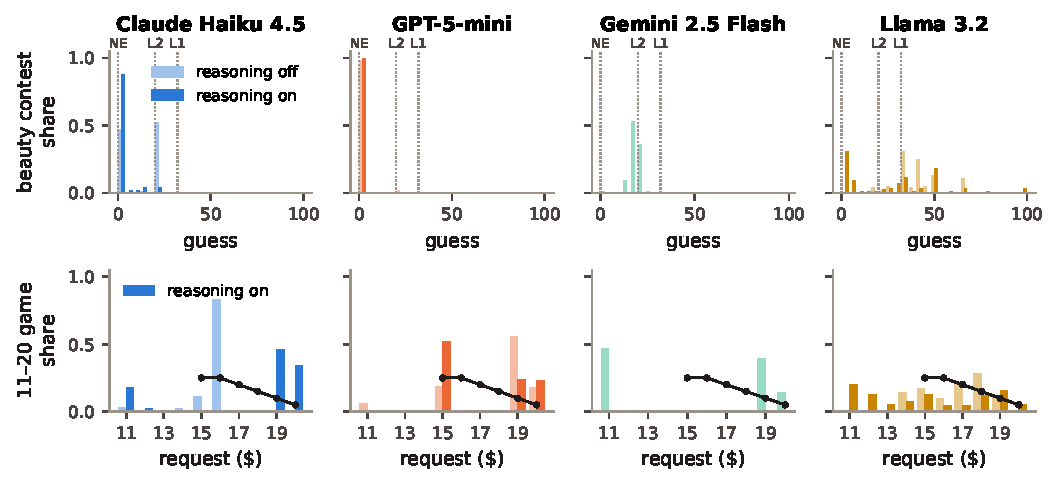
\includegraphics[width=\linewidth]{figs/fig1_choices.pdf}
\caption{Choices in the neutral framing, 100 calls per bar group. Top: beauty contest (bins of 4; dotted lines at NE and level-$k$ predictions). Bottom: 11--20 game (black line: equilibrium mix). Light bars: reasoning off; dark bars: on. Gemini was run with reasoning off only.}\label{fig:choices}
\end{figure}

\subsection{Fitted depth and its stability (RQ1)}
Table~\ref{tab:tau} gives the fitted depth in the neutral framing without visible reasoning, and Figure~\ref{fig:tau} all 49 conditions. No model is deep everywhere. Gemini has the largest $\tau$ of the four models in the beauty contest and the $3{\times}3$ game but one of the smallest in the 11--20 game; Haiku shows the reverse pattern. All 18 model pairs differ in their choice distributions, and the bootstrap interval of the $\tau$ difference excludes zero in 12 of them, so H1 (that $\tau$ differs between model families) is supported, but the ordering of models depends on the game. Across all 67 pre-registered comparisons, 48 show different choice distributions ($p<.05$) and 28 show different $\tau$.

\begin{table}[t]
\centering\small
\caption{Fitted depth $\hat\tau$ [95\% bootstrap interval] and equilibrium share $\hat\alpha$ (CH + equilibrium-type model), neutral framing, reasoning off, 99--100 valid choices each. $^\dagger$ the likelihood is flat up to the grid edge: estimate or upper bound within 0.1 of $\tau=6$ (not identified).}\label{tab:tau}
\begin{tabular}{@{}lccc@{}}
\toprule
Model & Beauty contest & 11--20 game & $3{\times}3$ game\\
\midrule
Claude Haiku 4.5 & 1.95 [1.95, 2.45], $\alpha=.45$ & 4.60 [4.60, 4.60] (mode 16) & 0.65 [0.65, 0.65] (all C)\\
GPT-5-mini & 1.95 [0.00, 1.95], $\alpha=.95$ & 0.50 [0.40, 5.90]$^\dagger$ & 1.70 [1.35, 2.05]\\
Gemini 2.5 Flash & 2.80 [2.80, 2.80] & 0.30 [0.20, 0.40] & 5.00 [3.95, 5.95]$^\dagger$\\
Llama 3.2 & 0.35 [0.20, 0.50] & 4.90 [2.25, 5.80], $\alpha=.50$ & 0.65 [0.65, 0.65]\\
\midrule
Pooled, all 14 conditions & 2.50 [1.35, 3.80], $\alpha=.55$ & 0.25 [0.15, 5.90]$^\dagger$ & 1.55 [1.05, 2.25]\\
\bottomrule
\end{tabular}
\end{table}

\begin{figure}[t]
\centering
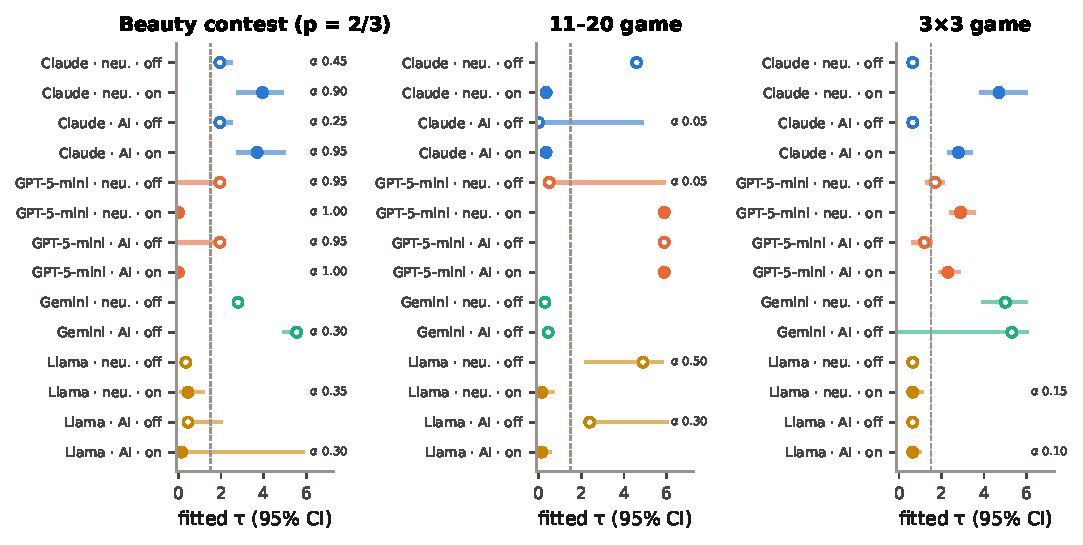
\includegraphics[width=\linewidth]{figs/fig2_tau.pdf}
\caption{$\hat\tau$ with 95\% bootstrap intervals for every condition (filled: reasoning on; open: off). $\alpha$ is shown where at least 0.05. The dashed line marks the typical human value $\tau\approx1.5$ \citep{camerer2004}.}\label{fig:tau}
\end{figure}

Pooling the 14 beauty-contest conditions, each counted as one player type, gives $\tau=2.50$ [1.35, 3.80] with an equilibrium share of $0.55$ [0.30, 0.75]. People typically have $\tau\approx1.5$ and rarely choose exactly 0 \citep{camerer2004,nagel1995}, so as a population these models play the equilibrium of a dominance-solvable game far more often than people do. Per-condition intervals are often degenerate (for example [1.95, 1.95]) because a near-deterministic model resamples to the same distribution; this reflects low variability between calls, not precision about a population, and is why the pooled fit is the more defensible summary.

\subsection{What moves the depth}
\paragraph{Visible reasoning.} In the true on/off comparison (Haiku, Llama) reasoning changed the choice distribution in all 14 cases; for GPT-5-mini, which reasons internally either way, visible reasoning changed 4 of 7, none in the beauty contest. The direction depended on the game. Where iterated dominance solves the game it moved play to the equilibrium: Haiku's share of guesses of 0 or 1 rose from 47\% to 88\% (neutral) and from 26\% to 91\% (AI framing), and its share of $A$ in the $3{\times}3$ game from 0--5\% to 78--95\%. In the 11--20 game, which has no dominance argument, reasoning made Haiku \emph{shallower}: its modal request moved from 16 (level 4) to 19 and 20 (levels 1 and 0). H2 is therefore supported for reasoning, with a game-dependent sign.

\paragraph{Framing.} Framing changed the distribution in 8 of 21 comparisons. Told it was an AI agent in a tournament, Gemini guessed lower in the beauty contest (guesses of 0 rose from 1\% to 19\%; $\hat\tau$ 2.80 $\to$ 5.55), and Haiku's modal 11--20 request moved from 16 to 11.

\paragraph{Misread equilibria and knowing versus playing.} Many requests of 11 in the 11--20 game do not reflect nine steps of reasoning. Asked to state the equilibrium, Haiku answered ``both request 11'' in two of three probes (and ``20'' in the third); it requests 11 in up to 39\% of calls, and Gemini in 29--46\%. Only GPT-5-mini stated the mixed equilibrium correctly (two of three probes, with exact probabilities). Conversely, knowing an equilibrium is not the same as playing it: Gemini stated that everyone should choose 0 in all three beauty-contest probes and then guessed around 18. That is the behavior level-$k$ predicts, a best response to beliefs that others do not play the equilibrium.

\subsection{Robustness of the fitted depth}
\paragraph{Level~0 (S2, S3).} Asked what a non-strategic player would choose, Haiku, GPT-5-mini and Gemini answered 50 in the beauty contest; in the 11--20 game GPT-5-mini answered 20, Haiku 15 and Gemini 20 or 15. With these answers as level~0 (S3), the beauty-contest $\tau$ barely moves (Haiku 1.95 $\to$ 2.45, Gemini 2.80 $\to$ 2.95, GPT-5-mini unchanged), so it is robust. In the 11--20 and $3{\times}3$ games it does not survive: GPT-5-mini's 11--20 $\tau$ falls from the grid edge to 0.60--0.75, and Haiku's moves 4.60 $\to$ 0.00 without reasoning and 0.35 $\to$ 5.65 with it. S2 (level~0 $=$ request 20) gives GPT-5-mini 0.40--0.75, confirming the pre-registered reading that a boundary $\tau$ in this game signals a focal level~0 rather than deep reasoning. Both imply the same level-1 action, 19, so the gap in $\hat\tau$ comes only from how requests of 20 are explained (level~0 under S2; tremble or level~0's one-in-ten chance under uniform). By the pre-registered rule, $\tau$ values for these two games are reported as level-0-dependent. The elicited level~0 fits better than the uniform one in 26 of 49 conditions.

\paragraph{The $p=\tfrac12$ control.} Gemini halved its guesses (mean 18.5 $\to$ 9.1, mode 10, which is level~2 at $p=\tfrac12$), suggesting computation; Llama ignored $p$ (60\% guessed 50). Because the equilibrium is 0 for both values of $p$, this control cannot separate computing the equilibrium from recalling it, which motivated E1.

\subsection{Extension E1: computing versus recalling the equilibrium}\label{sec:c30}
In the shifted contest (target $\tfrac23\times$mean $+30$) the equilibrium is 90 and the memorized answer 0 is poor. The pre-registered readings were: ``recall'' if at least 25\% of guesses are within 1 of 0, and ``equilibrium reasoning'' if at least 25\% are within 3 of 90. Table~\ref{tab:c30} and Figure~\ref{fig:c30} show the results.

\begin{table}[t]
\centering\small\setlength{\tabcolsep}{4pt}
\caption{Standard (NE 0) vs.\ shifted (NE 90) beauty contest, neutral framing, 100 calls per row (Llama with reasoning: 84 valid).}\label{tab:c30}
\begin{tabular}{@{}llccccl@{}}
\toprule
& & Standard & \multicolumn{4}{c}{Shifted (target $\tfrac23\times$mean $+30$)}\\
\cmidrule(lr){3-3}\cmidrule(lr){4-7}
Model & Reasoning & \% within 1 of 0 & \% within 1 of 0 & \% within 3 of 90 & mean & most frequent\\
\midrule
Haiku 4.5 & off & 47 & 0 & 0 & 35.2 & 30 (56), 36 (21)\\
Haiku 4.5 & on & 88 & 4 & 77 & 78.3 & 90 (77)\\
GPT-5-mini & off & 98 & 0 & 100 & 90.0 & 90 (100)\\
GPT-5-mini & on & 100 & 0 & 100 & 90.0 & 90 (100)\\
Gemini 2.5 Flash & off & 1 & 0 & 11 & 81.2 & 80, 85, 83, 78\\
Llama 3.2 & off & 0 & 0 & 0 & 46.9 & 43, 67, 42, 40\\
Llama 3.2 & on & 28 & 11 & 2 & 38.9 & 30, 50, 0\\
\bottomrule
\end{tabular}
\end{table}

\begin{figure}[t]
\centering
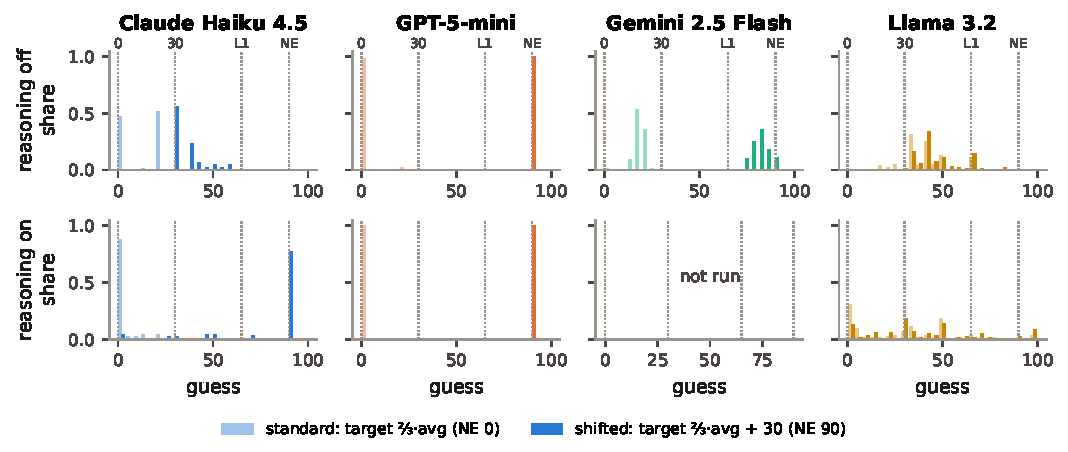
\includegraphics[width=\linewidth]{figs/fig3_c30.pdf}
\caption{Standard (light) and shifted (dark) beauty contest, neutral framing. Dotted lines: 0, 30 (the target if everyone guesses 0), level~1 of the shifted game (65) and its equilibrium (90).}\label{fig:c30}
\end{figure}

No condition meets the recall criterion. GPT-5-mini chose 90 in all 200 calls and stated 90 as the equilibrium in all three probes, so its near-universal 0 in the standard game is consistent with computing the equilibrium rather than simply recalling the textbook answer; the experiment cannot show the internal process. Haiku with reasoning behaved the same way (77\% at 90). Haiku without reasoning chose 30 in 56\% of calls: 30 is the target if everyone else guesses 0, so this is a best response to a memorized belief that others play the textbook answer, not a memorized action, and Haiku's probes also named 0 as the equilibrium in two of three answers. Gemini (78--85, levels 3--5; $\hat\tau=5.45$ [4.80, 6.00]) stated 90 in all probes but did not play it, as in the standard game. Llama stayed near the level-0 region. This is the clearest evidence in the study that the same model can reason, rely on a stored belief, or best-respond to beliefs about others depending on whether it reasons visibly.

\subsection{Exploiting the fitted depth offline (RQ2)}
Figure~\ref{fig:offline}a shows the gain over equilibrium play by round, averaged over the 14 replayed opponents. The CH exploiter is best at the start: in round~1 it gains \$4.74 per round over equilibrium play, against \$3.76 for fictitious play and $-\$1.67$ for regret matching, because the CH prior already tells it to undercut a shallow opponent. By rounds 4--5 fictitious play overtakes it, and over 20 rounds the mean gains are \$5.83 (fictitious play), \$5.43 (CH) and \$5.36 (regret matching), against \$6.87 for a best response to the true distribution. The CH exploiter reaches that ceiling against 6 of 14 opponents and falls behind where its model misfits: against GPT-5-mini in the AI framing, which requests 20 most often, it earns \$4.76--6.29 against a ceiling near \$10. An exploiter that uses level~0 $=$ request 20 earns \$9.90--10.41 against those two opponents but less on average (\$4.81), so the level-0 assumption matters for exploitation as much as for estimation.

Figure~\ref{fig:offline}b shows the safety trade-off. With online learning the gain is positive against every opponent at every $\epsilon$ (worst opponent: $+\$0.73$ at $\epsilon=0$). Committing to a wrong fixed $\tau'$ without learning loses up to \$4.90 per round at $\epsilon=0$; both quantities scale by $(1-\epsilon)$, as Section~\ref{sec:model} shows they must against a fixed opponent. Offline, H3 (some $\epsilon<1$ gives a significant gain at bounded worst-case loss) holds trivially: any $\epsilon$ trades gain for safety at the same rate. Offline replay, however, assumes the opponent never responds to the exploiter.

\begin{figure}[t]
\centering
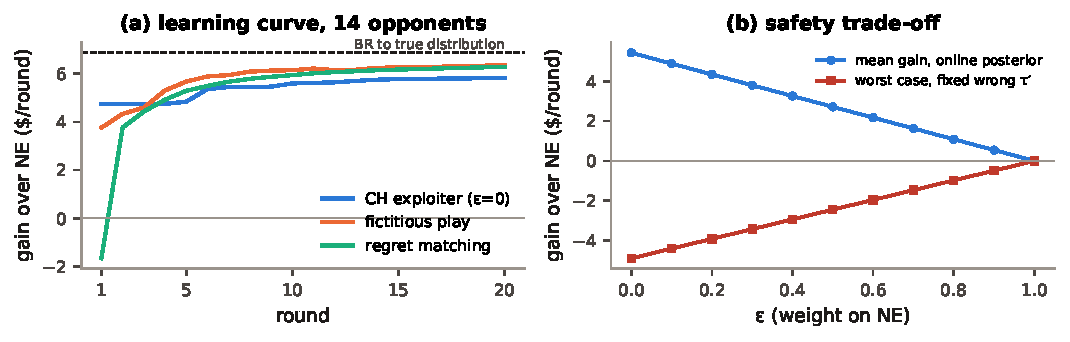
\includegraphics[width=\linewidth]{figs/fig4_offline.pdf}
\caption{Offline exploitation in the 11--20 game. (a) Gain over equilibrium play by round, mean over 14 replayed opponents, 300 matches each. (b) Mean gain with the online posterior and worst case with a fixed wrong $\tau'$, as $\epsilon$ varies.}\label{fig:offline}
\end{figure}

\subsection{Live exploitation and extension E2}\label{sec:live}
Table~\ref{tab:live} and Figure~\ref{fig:live} show the live matches. Pure exploitation ($\epsilon=0$) beats equilibrium play against all three models (\$1.70--3.56 per round). But GPT-5-mini learns: the $\epsilon=0$ exploiter's best response to its prior is to request 18 in the early rounds, GPT-5-mini learns to undercut it, and it out-earns the exploiter by \$6.41 per round [5.29, 7.59], with a hindsight regret of only \$1.18 per round (Haiku \$9.34, Llama \$14.65). Mixing in the equilibrium ($\epsilon=0.5$) removes the counter-exploitation (difference \$0.90 [$-0.90$, 2.91]) at the same gain over equilibrium play (\$1.62 vs.\ \$1.70), but against Haiku and Llama, which do not adapt, it gives up most of the gain (\$3.56 $\to$ 1.28; \$3.01 $\to$ 0.81). So the value of safety depends on whether the opponent learns, which offline replay cannot reveal. (A 5-match pilot suggested that Haiku also counter-exploits; with 15 matches it does not: \$1.11 [$-2.31$, 3.77].)

\begin{table}[t]
\centering\small
\caption{Live repeated 11--20 game: 15 matches $\times$ 10 rounds per cell, reasoning off. Values in \$ per round. 95\% intervals resample whole matches (the 10 rounds of a match are dependent), so they describe uncertainty across matches against the same model, not across models or prompts.}\label{tab:live}
\begin{tabular}{@{}llccc@{}}
\toprule
Opponent & Exploiter & Gain over NE play & LLM $-$ exploiter & LLM regret\\
\midrule
Haiku 4.5 & NE & 0.26 [$-0.64$, 1.07] & $-1.09$ [$-2.31$, 0.15] & 4.09\\
& $\epsilon=0.5$ & 1.28 [0.12, 2.36] & $-0.47$ [$-1.99$, 1.35] & 7.11\\
& $\epsilon=0$ & 3.56 [1.74, 5.88] & 1.11 [$-2.31$, 3.77] & 9.34\\
& adaptive & 1.54 [0.30, 2.92] & 1.63 [$-0.49$, 3.64] & 7.17\\
\midrule
GPT-5-mini & NE & $-0.87$ [$-1.59$, $-0.04$] & 1.57 [$-0.07$, 3.34] & 3.31\\
& $\epsilon=0.5$ & 1.62 [0.40, 2.76] & 0.90 [$-0.90$, 2.91] & 4.41\\
& $\epsilon=0$ & 1.70 [0.84, 2.59] & \textbf{6.41 [5.29, 7.59]} & 1.18\\
& adaptive & \textbf{2.74 [1.54, 3.94]} & 0.43 [$-1.10$, 1.92] & 2.60\\
\midrule
Llama 3.2 & NE & $-0.10$ [$-1.01$, 0.86] & $-0.02$ [$-1.47$, 1.49] & 4.18\\
& $\epsilon=0.5$ & 0.81 [$-0.20$, 1.92] & $-0.34$ [$-1.98$, 1.15] & 7.28\\
& $\epsilon=0$ & 3.01 [1.77, 4.25] & $-2.15$ [$-3.93$, $-0.40$] & 14.65\\
& adaptive & 2.83 [1.76, 4.11] & $-1.58$ [$-3.63$, 0.13] & 13.91\\
\bottomrule
\end{tabular}
\end{table}

\begin{figure}[t]
\centering
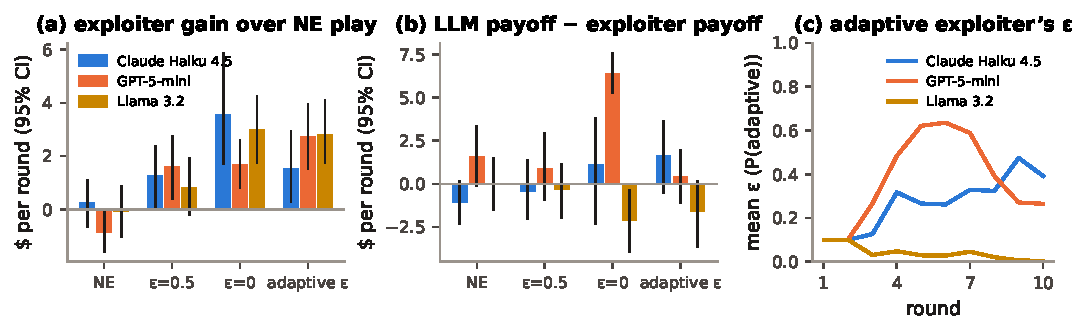
\includegraphics[width=\linewidth]{figs/fig5_live.pdf}
\caption{Live matches. (a) Exploiter's gain over equilibrium play. (b) LLM payoff minus exploiter payoff. (c) The adaptive exploiter's mean $\epsilon_t$ (its belief that the opponent is adapting) by round.}\label{fig:live}
\end{figure}

The adaptive-$\epsilon$ exploiter (E2) was pre-specified with the hypothesis that it would keep most of the $\epsilon=0$ gain against Haiku and Llama and remove GPT-5-mini's counter-exploitation. Against GPT-5-mini it gained the most of any strategy (\$2.74 [1.54, 3.94]) and the counter-exploitation disappeared (\$0.43 [$-1.10$, 1.92]); its $\epsilon_t$ rose to about 0.6 by rounds 5--6 and fell again once the opponent stopped undercutting (Figure~\ref{fig:live}c). Against Llama, $\epsilon_t$ stayed near 0 and the gain (\$2.83) was 94\% of pure exploitation. Against Haiku the hypothesis failed: Haiku's requests drift down by about one per round early in a match, which the detector partly read as adaptation ($\epsilon_t\approx0.3$), and the gain fell to \$1.54, less than half of pure exploitation's \$3.56. The hypothesis is therefore supported for two of three models. The adaptive matches were run four days after the other live matches and not interleaved with them, so a change in the served models cannot be ruled out.

\section{Discussion}
\paragraph{RQ1.} The CH parameter summarizes a model's play in a given condition, but not a model. The same model can be among the deepest players in one game and among the shallowest in another, and visible reasoning and framing move $\tau$ substantially. The pattern is interpretable through the course concepts: where iterated elimination of dominated strategies yields the equilibrium, these models can carry it out, often all the way, and reasoning helps; where the equilibrium requires mixing and there is no dominance chain (the 11--20 game), reasoning does not deepen play and models sometimes act on an incorrect equilibrium (``both request 11''). The shifted contest shows that the equilibrium play is often computed rather than recalled, and also shows a third mode, best-responding to a memorized belief about others. That the CH model fits only after adding an equilibrium type is itself a finding: LLM populations mix level-$k$ players with players who solve the game.

\paragraph{RQ2.} A fitted depth can be exploited: every exploiter that best-responds to the CH posterior beat equilibrium play against every LLM tested, offline and live. The model-based exploiter's advantage is in the first few rounds, before data accumulate; with more rounds, model-free learning matches or beats it, especially where the CH model misfits. The live experiment adds what offline analysis cannot: an LLM that adapts can turn a deterministic exploiter's best response against it. Detecting adaptation and setting $\epsilon$ accordingly recovers most of both benefits for two of three models.

\paragraph{Empirical findings and theoretical guarantees.} Three statements in this report are mathematical: iterated dominance and support enumeration give the equilibria in Table~\ref{tab:games}; against a fixed opponent the gain of the $\epsilon$-mixture is proportional to $1-\epsilon$; and regret matching's average regret vanishes asymptotically. Everything else is empirical. In particular, our exploiter has no safety guarantee in the sense of \citet{ganzfried2015}: the game is general-sum, equilibrium play is not maximin, and the opponents adapt.

\paragraph{Alternative explanations.} (i) \emph{Determinism instead of reasoning depth:} at temperature 1.0 some models return almost the same answer every time, so a ``population'' of 100 calls may reflect one decision rule plus sampling noise; the pooled fit and the choice-distribution tests are less sensitive to this than per-condition $\tau$. (ii) \emph{Recall:} the shifted contest and the probes rule out pure recall of an action for GPT-5-mini and Haiku with reasoning, but not recall of a solution method. (iii) \emph{Prompt sensitivity:} two framings are a small sample of possible wordings; framing effects of the size we found suggest other wordings would also move $\tau$.

\paragraph{Limitations and unsuccessful approaches.} The models are four small, low-cost models; results may differ for frontier models. $\tau$ outside the beauty contest depends on the level-0 definition. The equilibrium type was added after the pilot, and the two extensions after the main results; they were specified before their data, but they are exploratory. Live results rest on 15 matches per cell, which limits statistical power: differences under about \$2 per round are not reliably detected. Some matches against Haiku repeat almost exactly (6 distinct request sequences in 15 against $\epsilon=0$), so its matches are not independent draws of behavior and its intervals are too narrow; the live results speak to these three models under one prompt, not to LLMs in general. Unsuccessful approaches: the first pilot was lost to the gateway cache; Gemini's reasoning-on conditions could not be run within token limits; and the pre-registered model without an equilibrium type could not describe the dominant behavior in the beauty contest.

\section{Conclusion}
Large language models do not have a stable reasoning depth. Their cognitive-hierarchy depth depends on the game, the framing and whether they reason visibly; where iterated dominance solves the game they often compute the equilibrium, more often than people do, and where it does not, visible reasoning does not help and misread equilibria appear. Their depth can still be exploited, but an LLM that learns within a match can turn pure exploitation against the exploiter, so the safety margin of an $\epsilon$-safe exploiter is worth paying only against opponents that adapt. Useful next steps are frontier models and more framings, populations of LLMs playing each other, and an adaptive exploiter with a richer model of learning opponents. Code, prompts, raw logs and reproduction scripts: \codelink; recorded presentation: \videolink.

\begingroup\small
\bibliographystyle{plainnat}
\begin{thebibliography}{99}
\bibitem[Akata et~al.(2025)]{akata2025} E.~Akata, L.~Schulz, J.~Coda-Forno, S.~J. Oh, M.~Bethge, and E.~Schulz. Playing repeated games with large language models. \emph{Nature Human Behaviour}, 2025. arXiv:2305.16867.
\bibitem[Alekseenko et~al.(2025)]{alekseenko2025} I.~Alekseenko, D.~Dagaev, S.~Paklina, and P.~Parshakov. Strategizing with AI: Insights from a beauty contest experiment. arXiv:2502.03158, 2025.
\bibitem[Arad and Rubinstein(2012)]{arad2012} A.~Arad and A.~Rubinstein. The 11--20 money request game: A level-$k$ reasoning study. \emph{American Economic Review}, 102(7):3561--3573, 2012.
\bibitem[Brown(1951)]{brown1951} G.~W. Brown. Iterative solution of games by fictitious play. In T.~C. Koopmans, editor, \emph{Activity Analysis of Production and Allocation}, pages 374--376. Wiley, 1951.
\bibitem[Camerer et~al.(2004)]{camerer2004} C.~F. Camerer, T.-H. Ho, and J.-K. Chong. A cognitive hierarchy model of games. \emph{Quarterly Journal of Economics}, 119(3):861--898, 2004.
\bibitem[Crawford et~al.(2013)]{crawford2013} V.~P. Crawford, M.~A. Costa-Gomes, and N.~Iriberri. Structural models of nonequilibrium strategic thinking: Theory, evidence, and applications. \emph{Journal of Economic Literature}, 51(1):5--62, 2013.
\bibitem[Duan et~al.(2024)]{duan2024} J.~Duan et~al. GTBench: Uncovering the strategic reasoning limitations of LLMs via game-theoretic evaluations. In \emph{Advances in Neural Information Processing Systems (NeurIPS)}, 2024. arXiv:2402.12348.
\bibitem[Efron and Tibshirani(1993)]{efron1993} B.~Efron and R.~J. Tibshirani. \emph{An Introduction to the Bootstrap}. Chapman \& Hall, 1993.
\bibitem[Gandhi et~al.(2023)]{gandhi2023} K.~Gandhi, D.~Sadigh, and N.~D. Goodman. Strategic reasoning with language models. arXiv:2305.19165, 2023.
\bibitem[Ganzfried and Sandholm(2015)]{ganzfried2015} S.~Ganzfried and T.~Sandholm. Safe opponent exploitation. \emph{ACM Transactions on Economics and Computation}, 3(2):8:1--8:28, 2015.
\bibitem[Guo(2023)]{guo2023} F.~Guo. GPT in game theory experiments. arXiv:2305.05516, 2023.
\bibitem[Hart and Mas-Colell(2000)]{hart2000} S.~Hart and A.~Mas-Colell. A simple adaptive procedure leading to correlated equilibrium. \emph{Econometrica}, 68(5):1127--1150, 2000.
\bibitem[Ho et~al.(1998)]{ho1998} T.-H. Ho, C.~Camerer, and K.~Weigelt. Iterated dominance and iterated best response in experimental ``$p$-beauty contests''. \emph{American Economic Review}, 88(4):947--969, 1998.
\bibitem[Johanson et~al.(2008)]{johanson2008} M.~Johanson, M.~Zinkevich, and M.~Bowling. Computing robust counter-strategies. In \emph{Advances in Neural Information Processing Systems 20 (NIPS 2007)}, pages 721--728, 2008.
\bibitem[McKelvey and Palfrey(1995)]{mckelvey1995} R.~D. McKelvey and T.~R. Palfrey. Quantal response equilibria for normal form games. \emph{Games and Economic Behavior}, 10(1):6--38, 1995.
\bibitem[Nagel(1995)]{nagel1995} R.~Nagel. Unraveling in guessing games: An experimental study. \emph{American Economic Review}, 85(5):1313--1326, 1995.
\bibitem[Stahl and Wilson(1995)]{stahl1995} D.~O. Stahl and P.~W. Wilson. On players' models of other players: Theory and experimental evidence. \emph{Games and Economic Behavior}, 10(1):218--254, 1995.
\bibitem[Wang et~al.(2026)]{wang2026} Z.~Wang, I.~Ahmed, P.~Unjitwattana, E.~Y. Xie, M.-J. Fong, and P.-H. Lin. Revisiting the intra-team communication method to elicit level-$k$ reasoning in beauty contests and 11--20 games. arXiv:2608.18069, 2026.
\bibitem[Wellman(2006)]{wellman2006} M.~P. Wellman. Methods for empirical game-theoretic analysis. In \emph{Proceedings of the 21st National Conference on Artificial Intelligence (AAAI)}, pages 1552--1555, 2006.
\bibitem[Zhang et~al.(2025)]{zhang2025} Y.~Zhang, S.~Mao, T.~Ge, X.~Wang, Y.~Xia, M.~Lan, and F.~Wei. K-level reasoning: Establishing higher order beliefs in large language models for strategic reasoning. In \emph{Proceedings of NAACL}, 2025. arXiv:2402.01521.
\end{thebibliography}
\endgroup

\clearpage
\appendix
\section{Reproducibility}\label{app:repro}
\paragraph{Code and data.} \codelink. The archive contains the sampling harness (\texttt{harness/}), the analysis code (\texttt{analysis/}), every raw log (\texttt{data/*.jsonl}: prompt identifier, raw reply, hidden-reasoning text where returned, served model, token usage, latency, session code and UTC timestamp for every call), the pre-registration and its dated deviations, and a README. Results in this report correspond to \commitref.

\sloppy
\paragraph{Software.} Analysis: Python 3.13, NumPy 2.5.3, SciPy 1.18.1, pandas 3.0.5, Matplotlib 3.11.2 (pinned in \texttt{requirements.txt}). Data collection: the \texttt{openai} Python client with streaming calls, as the gateway requires (version \openaiversion). Fitting code: \texttt{levelk.py} (model), \texttt{fit.py} (per-condition fits and bootstrap), \texttt{pooled.py} (population fit), \texttt{tests.py} (67 comparisons), \texttt{phase2.py} (offline exploitation), \texttt{run\_live.py} (live summaries), \texttt{run\_s3.py}, \texttt{run\_c30.py}, \texttt{figs\_report.py}.

\paragraph{Models and settings.} Gateway \texttt{https://chat.tamu.ai/api}; identifiers \texttt{protected.Claude-Haiku-4.5}, \texttt{protected.gpt-5-mini}, \texttt{protected.gemini-2.5-flash}, \texttt{protected.llama3.2}; temperature 1.0 for all models; no API seed (the gateway's handling of seeds is undocumented); maximum output tokens 4{,}096 (reasoning off) and 8{,}192 (on), and 8{,}192/16{,}384 for GPT-5-mini. Each call is stateless: a system message \texttt{Session code: <8 random letters>} and one user message. Live matches resend the full history each round. Call dates: pilots Nov~4; main run and $p=\tfrac12$ Nov~18; live matches Nov~18--19; level-0 elicitation Nov~19; shifted contest and adaptive matches Nov~22, 2026.

\paragraph{Trials and randomness.} 100 calls per condition; the order of calls is shuffled across conditions (seed 631) so that drift or outages do not fall on one condition. Bootstrap and simulation seed 631; the exploiter's random draws in match $k$ use seed $\mathrm{crc32}(\text{model}|\text{strategy}|k)$. Invalid replies (no \texttt{ANSWER} line or out of range) are excluded and counted: 48 of 4{,}900 in the main run including the $p=\tfrac12$ control, 16 of 700 in the shifted contest (all Llama with reasoning), 0 of 1{,}800 live.

\paragraph{Commands.} Data collection, run inside \texttt{harness/} with \texttt{TAMU\_API\_KEY} and \texttt{TAMU\_COOKIE} set:
\begin{quote}\small\ttfamily\raggedright
cd harness\\
python3 harness.py run --models <ids> --games beauty req11\_20 matrix3x3 --framings neutral ai\_competition --cot off on --n 100 --out main.jsonl\\
python3 live\_1120.py --models <ids> --strategies ne exploit5 exploit0 adaptive --matches 15 --rounds 10 --out live\_1120.jsonl
\end{quote}
Every table and figure from the logs, without API calls, run from the archive root:
\begin{quote}\small\ttfamily\raggedright
pip install -r requirements.txt; export PYTHONPATH=analysis\\
python3 analysis/run\_main.py; python3 analysis/tests.py; python3 analysis/run\_pooled.py\\
python3 analysis/run\_s3.py; python3 analysis/run\_c30.py; python3 analysis/run\_live.py\\
python3 analysis/phase2.py results/p2 data/main\_haiku.jsonl data/main\_gpt.jsonl data/main\_gemini.jsonl data/main\_llama.jsonl --R 20 --M 300\\
python3 analysis/figs\_report.py
\end{quote}

\paragraph{Budget.} 8{,}448 logged calls in total (main run 4{,}200, $p=\tfrac12$ control 700, shifted contest 700, level-0 elicitation 360, Nash probes 48, live 1{,}800, pilots 640). Not logged: automatic retries after transient gateway errors (the harness retries up to four times and logs only the final outcome) and about 30 connectivity and cache-test calls; \$18.68 at public list prices: main run \$11.48 (Gemini \$5.31), $p=\tfrac12$ control \$1.48, shifted contest \$1.72, level-0 elicitation \$0.61, live matches \$1.20 and pilots \$2.19. The Nash probes (48 short calls) did not log token usage and are not included. All of this was within the course gateway's daily limit. Llama~3.2 is free. Token use differed sharply across models because GPT-5-mini and Gemini reason internally.

\paragraph{Limits on reproducibility.} The models are hosted and may be updated without notice, so new runs will not reproduce the exact choices; the logs allow every table and figure to be reproduced exactly from the recorded data. The gateway's cache means that runs without a session code are not independent samples.

\section{Prompts}\label{app:prompts}
Every call has a system message \texttt{Session code: <8 random letters>} and one user message. \textbf{Beauty contest, neutral framing, reasoning off} (the other games replace the middle paragraph with the rules below):
\begin{quote}\small\ttfamily\raggedright
You are a participant in a decision-making study. You will play a game once.\\[3pt]
There are 7 players: you and 6 other participants. Each player privately chooses a whole number from 0 to 100 (inclusive). The winner is the player whose number is closest to 2/3 of the average of all 7 chosen numbers, including their own. The winner receives \$10; if several players tie, they split the \$10. Everyone else receives nothing.\\[3pt]
Which number do you choose?\\[3pt]
Do not explain your reasoning. Reply with exactly one line of the form\\ ANSWER: <a whole number from 0 to 100>
\end{quote}
\begin{itemize}\small
\item \textbf{AI framing:} the first line becomes \emph{``You are an AI agent competing in a tournament against other AI agents. You will play a game once.''} and ``other participants'' becomes ``other AI agents''.
\item \textbf{Reasoning on:} the last instruction becomes \emph{``Think through the problem step by step. Then end your reply with a final line of the form ANSWER: <\dots>''}.
\item \textbf{$p=\tfrac12$ and shifted contest:} ``1/2 of the average'', or ``2/3 of the average of all 7 chosen numbers (including their own) plus 30''.
\item \textbf{11--20 game:} \emph{``You and one other participant each request an amount of money. The amount must be a whole number of dollars from 11 to 20 (inclusive). Each of you receives the amount you requested. In addition, if your request is exactly one dollar less than the other's request, you receive an extra \$20. How much do you request?''}
\item \textbf{$3{\times}3$ game:} \emph{``You and one other participant each choose one action: A, B or C. You choose at the same time without seeing the other's choice. The other player faces exactly the same table. Your payoff in dollars: If you choose A: \$10 if they choose A, \$0 if they choose B, \$9 if they choose C. [B: 5, 6, 0; C: 9, 10, 6.] Which action do you choose?''}
\item \textbf{Nash probe:} the game text, then \emph{``Do not choose an action. Instead, state what game theory predicts: describe the Nash equilibrium of this game (pure or mixed) in at most three sentences. End with a final line NASH: <your short answer>''}.
\item \textbf{Level-0 elicitation:} the game text, then \emph{``Do not choose for yourself. Instead, imagine another player who does not think about what the other players will do and chooses without any strategic reasoning. What would such a player most likely choose?''} and the reasoning-off instruction.
\item \textbf{Live round $t$:} \emph{``You will play the same game with the same other participant for 10 rounds.''}, the 11--20 rules, \emph{``Results so far: -- Round 1: you requested \$19, the other requested \$18; you earned \$19, they earned \$38. [\dots] This is round $t$ of 10. How much do you request?''} and the reasoning-off instruction.
\end{itemize}

\section{All fitted conditions}\label{app:cells}
\footnotesize
\setlength{\tabcolsep}{1.8pt}
\begin{longtable}{@{}llllrrp{2.3cm}lrlrr@{}}
\caption{Every condition: valid choices $n$, number of distinct choices, the most frequent choices (value$\times$count), the level-$k$ type (uniform level~0) or equilibrium (NE) that predicts the single most frequent choice, $\hat\tau$ of the pre-registered model (Pre), and $\hat\tau$ [95\% CI], $\hat\alpha$, $\hat\delta$ (tremble) of the CH + equilibrium-type model. $^\dagger$ within 0.1 of the grid edge.}\label{tab:all}\\
\toprule
Game & Model & Framing & CoT & $n$ & Dist. & Most frequent & Level & Pre $\hat\tau$ & $\hat\tau$ [95\% CI] & $\hat\alpha$ & $\hat\delta$\\
\midrule\endfirsthead
\toprule
Game & Model & Framing & CoT & $n$ & Dist. & Most frequent & Level & Pre $\hat\tau$ & $\hat\tau$ [95\% CI] & $\hat\alpha$ & $\hat\delta$\\
\midrule\endhead
Beauty $p{=}2/3$ & Haiku 4.5 & neutral & off & 100 & 6 & 22$\times$48, 0$\times$43, 1$\times$4, 23$\times$3 & L2 & 1.80 & 1.95 [1.95, 2.45] & 0.45 & 0.00 \\
Beauty $p{=}2/3$ & Haiku 4.5 & neutral & on & 100 & 10 & 0$\times$87, 20$\times$3, 13$\times$2, 15$\times$2 & NE & 0.00 & 3.95 [2.80, 4.85] & 0.90 & 0.00 \\
Beauty $p{=}2/3$ & Haiku 4.5 & AI & off & 100 & 5 & 22$\times$72, 1$\times$20, 0$\times$6, 15$\times$1 & L2 & 1.80 & 1.95 [1.95, 2.45] & 0.25 & 0.00 \\
Beauty $p{=}2/3$ & Haiku 4.5 & AI & on & 100 & 6 & 0$\times$91, 5$\times$3, 15$\times$3, 10$\times$1 & NE & 0.00 & 3.70 [2.80, 4.95] & 0.95 & 0.00 \\
Beauty $p{=}2/3$ & GPT-5-mini & neutral & off & 100 & 2 & 0$\times$98, 22$\times$2 & NE & 0.00 & 1.95 [0.00, 1.95] & 0.95 & 0.00 \\
Beauty $p{=}2/3$ & GPT-5-mini & neutral & on & 100 & 1 & 0$\times$100 & NE & 0.00 & 0.00 [0.00, 0.00] & 1.00 & 0.00 \\
Beauty $p{=}2/3$ & GPT-5-mini & AI & off & 100 & 2 & 0$\times$99, 22$\times$1 & NE & 0.00 & 1.95 [0.00, 1.95] & 0.95 & 0.00 \\
Beauty $p{=}2/3$ & GPT-5-mini & AI & on & 100 & 1 & 0$\times$100 & NE & 0.00 & 0.00 [0.00, 0.00] & 1.00 & 0.00 \\
Beauty $p{=}2/3$ & Gemini 2.5 Fl. & neutral & off & 100 & 13 & 18$\times$18, 19$\times$16, 20$\times$15, 17$\times$14 & L2 & 2.80 & 2.80 [2.80, 2.80] & 0.00 & 0.00 \\
Beauty $p{=}2/3$ & Gemini 2.5 Fl. & AI & off & 100 & 18 & 0$\times$19, 13$\times$14, 15$\times$12, 8$\times$9 & NE & 6.00 & 5.55 [4.95, 5.70] & 0.30 & 0.00 \\
Beauty $p{=}2/3$ & Llama 3.2 & neutral & off & 100 & 19 & 33$\times$21, 42$\times$14, 50$\times$12, 34$\times$10 & L1 & 0.35 & 0.35 [0.20, 0.50] & 0.00 & 0.00 \\
Beauty $p{=}2/3$ & Llama 3.2 & neutral & on & 87 & 28 & 0$\times$19, 50$\times$15, 33$\times$6, 1$\times$5 & NE & 0.15 & 0.45 [0.15, 1.15] & 0.35 & 0.15 \\
Beauty $p{=}2/3$ & Llama 3.2 & AI & off & 100 & 24 & 33$\times$23, 34$\times$11, 42$\times$10, 16$\times$7 & L1 & 0.45 & 0.45 [0.30, 2.00] & 0.00 & 0.00 \\
Beauty $p{=}2/3$ & Llama 3.2 & AI & on & 93 & 34 & 50$\times$14, 0$\times$12, 100$\times$6, 3$\times$5 & none & 0.05 & 0.15 [0.05, 5.85] & 0.30 & 0.15 \\
Beauty $p{=}1/2$ & Haiku 4.5 & neutral & off & 100 & 5 & 0$\times$81, 22$\times$8, 13$\times$7, 25$\times$3 & NE & 6.00 & 1.60 [1.10, 1.90] & 0.80 & 0.00 \\
Beauty $p{=}1/2$ & Haiku 4.5 & neutral & on & 100 & 7 & 0$\times$90, 5$\times$4, 13$\times$2, 7$\times$1 & NE & 6.00 & 2.50 [0.00, 3.32] & 0.95 & 0.00 \\
Beauty $p{=}1/2$ & GPT-5-mini & neutral & off & 100 & 2 & 0$\times$99, 17$\times$1 & NE & 6.00 & 1.35 [0.00, 1.35] & 0.95 & 0.00 \\
Beauty $p{=}1/2$ & GPT-5-mini & neutral & on & 100 & 1 & 0$\times$100 & NE & 6.00 & 0.00 [0.00, 0.00] & 1.00 & 0.00 \\
Beauty $p{=}1/2$ & Gemini 2.5 Fl. & neutral & off & 100 & 10 & 10$\times$32, 9$\times$20, 6$\times$10, 7$\times$10 & L2 & 3.55 & 3.55 [3.30, 3.95] & 0.00 & 0.00 \\
Beauty $p{=}1/2$ & Llama 3.2 & neutral & off & 100 & 16 & 50$\times$60, 51$\times$7, 49$\times$5, 34$\times$5 & none & 0.00 & 0.00 [0.00, 0.00] & 0.00 & 0.00 \\
Beauty $p{=}1/2$ & Llama 3.2 & neutral & on & 89 & 22 & 50$\times$34, 0$\times$17, 7$\times$6, 25$\times$4 & none & 6.00 & 0.05 [0.00, 1.60] & 0.25 & 0.50 \\
11--20 & Haiku 4.5 & neutral & off & 100 & 5 & 16$\times$83, 15$\times$11, 11$\times$3, 14$\times$2 & L4 & 4.60 & 4.60 [4.60, 4.60] & 0.00 & 0.10 \\
11--20 & Haiku 4.5 & neutral & on & 100 & 4 & 19$\times$46, 20$\times$34, 11$\times$18, 12$\times$2 & L1 & 0.35 & 0.35 [0.25, 0.45] & 0.00 & 0.00 \\
11--20 & Haiku 4.5 & AI & off & 100 & 7 & 11$\times$39, 16$\times$29, 15$\times$13, 12$\times$6 & L9 & 0.00 & 0.00 [0.00, 4.85] & 0.05 & 0.10 \\
11--20 & Haiku 4.5 & AI & on & 100 & 4 & 19$\times$43, 20$\times$27, 11$\times$25, 12$\times$5 & L1 & 0.35 & 0.35 [0.25, 0.40] & 0.00 & 0.00 \\
11--20 & GPT-5-mini & neutral & off & 100 & 5 & 19$\times$56, 15$\times$19, 20$\times$18, 11$\times$6 & L1 & 0.45 & 0.50 [0.40, 5.90]$^\dagger$ & 0.05 & 0.00 \\
11--20 & GPT-5-mini & neutral & on & 100 & 4 & 15$\times$52, 19$\times$24, 20$\times$23, 11$\times$1 & L5 & 5.90 & 5.90 [5.90, 5.90]$^\dagger$ & 0.00 & 0.05 \\
11--20 & GPT-5-mini & AI & off & 100 & 5 & 20$\times$52, 19$\times$36, 15$\times$8, 11$\times$3 & L0 & 5.90 & 5.90 [5.90, 5.90]$^\dagger$ & 0.00 & 0.05 \\
11--20 & GPT-5-mini & AI & on & 100 & 3 & 20$\times$47, 15$\times$27, 19$\times$26 & L0 & 5.90 & 5.90 [5.90, 5.90]$^\dagger$ & 0.00 & 0.00 \\
11--20 & Gemini 2.5 Fl. & neutral & off & 99 & 3 & 11$\times$46, 19$\times$39, 20$\times$14 & L9 & 0.30 & 0.30 [0.20, 0.40] & 0.00 & 0.00 \\
11--20 & Gemini 2.5 Fl. & AI & off & 99 & 3 & 19$\times$55, 11$\times$29, 20$\times$15 & L1 & 0.45 & 0.45 [0.35, 0.55] & 0.00 & 0.00 \\
11--20 & Llama 3.2 & neutral & off & 100 & 6 & 18$\times$28, 17$\times$20, 15$\times$17, 14$\times$14 & L2 & 4.90 & 4.90 [2.25, 5.80] & 0.50 & 0.00 \\
11--20 & Llama 3.2 & neutral & on & 94 & 10 & 11$\times$19, 19$\times$15, 15$\times$12, 12$\times$12 & L9 & 0.15 & 0.15 [0.00, 0.65] & 0.00 & 0.45 \\
11--20 & Llama 3.2 & AI & off & 100 & 6 & 17$\times$29, 19$\times$20, 18$\times$17, 15$\times$13 & L3 & 2.50 & 2.40 [2.30, 6.00]$^\dagger$ & 0.30 & 0.15 \\
11--20 & Llama 3.2 & AI & on & 94 & 10 & 11$\times$22, 19$\times$18, 20$\times$12, 18$\times$9 & L9 & 0.15 & 0.15 [0.05, 0.55] & 0.00 & 0.20 \\
$3{\times}3$ & Haiku 4.5 & neutral & off & 100 & 1 & C$\times$100 & L1 & 0.65 & 0.65 [0.65, 0.65] & 0.00 & 0.00 \\
$3{\times}3$ & Haiku 4.5 & neutral & on & 100 & 2 & A$\times$95, C$\times$5 & NE (L2+) & 4.70 & 4.70 [3.85, 5.95]$^\dagger$ & 0.00 & 0.00 \\
$3{\times}3$ & Haiku 4.5 & AI & off & 100 & 2 & C$\times$95, A$\times$5 & L1 & 0.65 & 0.65 [0.65, 0.65] & 0.00 & 0.00 \\
$3{\times}3$ & Haiku 4.5 & AI & on & 100 & 2 & A$\times$78, C$\times$22 & NE (L2+) & 2.80 & 2.80 [2.35, 3.40] & 0.00 & 0.00 \\
$3{\times}3$ & GPT-5-mini & neutral & off & 100 & 2 & A$\times$53, C$\times$47 & NE (L2+) & 1.70 & 1.70 [1.35, 2.05] & 0.00 & 0.00 \\
$3{\times}3$ & GPT-5-mini & neutral & on & 99 & 2 & A$\times$79, C$\times$20 & NE (L2+) & 2.90 & 2.90 [2.45, 3.50] & 0.00 & 0.00 \\
$3{\times}3$ & GPT-5-mini & AI & off & 100 & 2 & C$\times$63, A$\times$37 & L1 & 1.20 & 1.20 [0.65, 1.50] & 0.00 & 0.00 \\
$3{\times}3$ & GPT-5-mini & AI & on & 100 & 2 & A$\times$69, C$\times$31 & NE (L2+) & 2.30 & 2.30 [1.95, 2.80] & 0.00 & 0.00 \\
$3{\times}3$ & Gemini 2.5 Fl. & neutral & off & 100 & 2 & A$\times$96, C$\times$4 & NE (L2+) & 5.00 & 5.00 [3.95, 5.95]$^\dagger$ & 0.00 & 0.00 \\
$3{\times}3$ & Gemini 2.5 Fl. & AI & off & 99 & 2 & A$\times$96, C$\times$3 & NE (L2+) & 5.30 & 5.30 [0.00, 6.00]$^\dagger$ & 0.00 & 0.00 \\
$3{\times}3$ & Llama 3.2 & neutral & off & 100 & 3 & C$\times$80, A$\times$17, B$\times$3 & L1 & 0.65 & 0.65 [0.65, 0.65] & 0.00 & 0.00 \\
$3{\times}3$ & Llama 3.2 & neutral & on & 99 & 3 & C$\times$58, A$\times$30, B$\times$11 & L1 & 0.80 & 0.65 [0.60, 1.10] & 0.15 & 0.00 \\
$3{\times}3$ & Llama 3.2 & AI & off & 100 & 3 & C$\times$74, A$\times$18, B$\times$8 & L1 & 0.65 & 0.65 [0.65, 0.65] & 0.00 & 0.00 \\
$3{\times}3$ & Llama 3.2 & AI & on & 100 & 3 & C$\times$55, A$\times$29, B$\times$16 & L1 & 0.70 & 0.65 [0.45, 1.00] & 0.10 & 0.05 \\
\bottomrule
\end{longtable}
\normalsize

\section{Pre-registration and deviations}\label{app:dev}
\begin{itemize}
\item \textbf{Nov 4, before any data:} level~0, matching and tie rules, games, grid, bootstrap and tests (Section~\ref{sec:model}); validation on synthetic agents.
\item \textbf{D1, after pilot 1:} random session code on every call (gateway cache); parser accepts a ``\$'' before the number; higher token limits; pilot~1 discarded.
\item \textbf{D2, after pilot 2:} equilibrium type $\alpha$ added; the pre-registered model is reported alongside.
\item \textbf{D3, after pilot 2:} Gemini reasoning-on conditions dropped; GPT-5-mini and Gemini treated as reasoning internally.
\item \textbf{D4, Nov 17, before the main run:} main-run design; GPT-5-mini token limits; population fit; offline and live exploitation protocols.
\item \textbf{D5, Nov 22, before their data:} extensions E1 (shifted contest, with recall and equilibrium criteria) and E2 (adaptive $\epsilon$, with its hypothesis).
\end{itemize}
Pilot~2 (320 calls) was used only for the progress report; no estimate here uses pilot data.

\end{document}
